 \documentclass[h]{article}
\usepackage[margin=0.5in]{geometry}
\usepackage{amsfonts} 
\usepackage{textcomp}
 
\usepackage{graphicx}
\usepackage{caption}
\usepackage{subcaption}
\usepackage{float} 
\usepackage{flafter}
\graphicspath{ {../images/} }
\usepackage{adjustbox}


\newcommand{\cent}{\textcent \hspace{4pt}}
\title{CS 7641 Machine Learning \\ Assignment 1}
\date{Due February 4th, 2018 11:59pm}
\author{Philip Bale \\ pbale3}

\begin{document}

\maketitle
2 most important plots: learning curve and model complexity curve

\section*{Classification Problems}
\subsection*{1) US Permanent Visa Applications}  
\subsubsection*{Overview}
The first classification problem revolves around classifying whether or not a 
person's US permanent visa application will be accepted or denied based on the parameters of 
their application.  Among the features used in the classifcation are:
\begin{itemize}
  \item Job features: Industry code, job class, wage rate, wage type
  \item Geographic features: Country of citizen and employer location
\end{itemize}
The classes observed for this dataset are simply 'approved' and 'denied'.  The 
dataset contains 374365 total samples.
\subsubsection*{Why is the dataset interesting?}
This dataset is interesting due to its potential to aid in the visa application 
process from a cost and time savings potential.  It could also enable confidence in those 
interested in applying for a US permanent visa but doubting their chances of 
acceptance.  At the end of the day, the goal is it to try to determine the application result 
before time, money, and other resources are spent.  As someone who has worked 
with a large number of first-generation visa holders and immigrants, I am 
extremely interested in building tools to help others to achieve the same.
\\ \\
From a machine learning perspective, the dataset is incredibly interesting due 
to its wide variety of features and the variety of values those features can take. 
 An immense number of job types, wage rates, and citizenships alone create an 
 extremely diverse dataset.  Additionally, the number of samples available 
 provide a comprehensive picture of historical data, lending towards greater 
 cofidence in training and testing rates.

\subsection*{2) Home Sale Price Predictions}  
\subsubsection*{Overview}
The second classification problem revolves around classifying a home's price 
bracket based upon the various characteristics of the home.  Among the features 
used in the classification are :
\begin{itemize}
  \item Subjective measurements: Exterior condition, house style, overall quality rating, and overall condition
  \item Objective measurements: Type of dwelling, building type, lot size, neighborhood, year built, and year sold
\end{itemize}
After an initial review of the dataset, the classes were defined as pricing 
brackets divided into 100k groups.  I.e: 0-100k, 100k-200k, 200k-300k, etc.  The 
dataset contains 1451 samples.  An additional dataset containing another 1400 
testing samples exists but was not used as it contains unclassified sale 
prices.  It will, however, prove useful for unsupervised learning.
\subsubsection*{Why is the dataset interesting?}
This dataset is interesting for two primary reasons: real-world applicability 
and participating in a Kaggle challenge.  First, modeling home prices is both a 
difficult and lucrative task.  If one can succesfully model home sale prices on 
large sets of data, he/she can make large amounts of money investing in real 
estate when he/she detects outliers in listed price vs. what it is expected to sell for.  
This applies to flipping, investing, and remodeling.  Second, the dataset is 
part of an ongoing Kaggle competition that does not have a winning solution yet. 
 By taking part of the competition, the dataset presents the opportunity to work 
 towards a winning solution and advance ones algorithms over time. 
 \\ \\
 Houses can have a very large amount of features--with a large amount of variety 
 in the individual features.  Similarly, housing is prone to personal taste and 
 frequent need for upgrades/modernization.  In such, I believe price estimation is an 
 excellent problem, full of depth and complexity, that is suitable for a machine 
 learning approach.
 
  \section*{General Data Processing}
  The datasets I used were both relatively clean to begin with.  One small 
  problem, however, was that a lot of my features on both datasets were 
  text-based.  To transform the features into numeric values suitable for the 
  machine learning algorithms, I used a label encoder built into ScikitLearn.
  \\ \\
  I also did a small amount of preprocessing of the data to make it more 
  suitable for classification.  I dropped all unnecessary columns to help 
  speed up with data processing in general--which proved immensely helpful when 
  dealing with the more computationall intensive algorithms.  In the 
  case of home prices, I precalculated the brackets based on the 'sale price' data label.  
  In the case of visa applications, I pregrouped the case outcome so that 
  results such as 'certified' and 'certified withdrawn' are both concerned as 
  'approved' conditions whereas 'denied', 'invalidated', and 'rejected' all 
  resolve to 'denied'.
  
 \section*{Decision Trees}
 A decision tree classifier was the first algorithm applied to the datsets.  
 Various values of max\_depth were tested as a means of pruning unnecessary 
 leaves.  Similarly, a grid search was used to test whether a 'gini' or 
 'entropy' criterion was more effective.

\subsection*{US Permanent Visa}

\begin{figure}[H]
    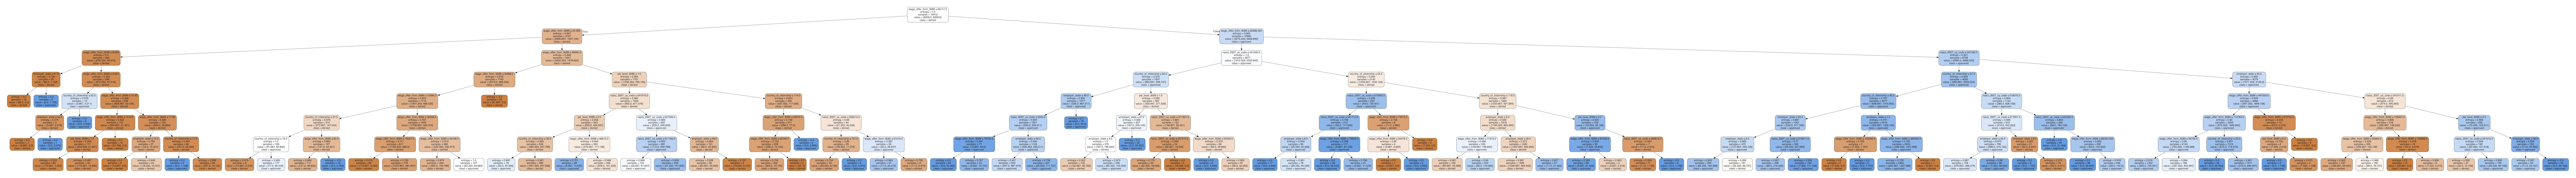
\includegraphics[width=1.0\textwidth,keepaspectratio]{1_dtree.jpg} 
    \caption*{Permanent Visa Decision Tree with max\_depth of 7} 
\end{figure}

\begin{tabular}{ | c | c  | c | c | c | c | c |} 
\hline
\textbf{Max Depth} & \textbf{Criterion} & \textbf{Tree Size} & \textbf{Train \%} & \textbf{Train runtime} & \textbf{Test \%} & \textbf{Test runtime}   \\
\hline
1 & gini & 3 & 0.7657 & 0.1212 & 0.7680 & 0.0010 \\ \hline
3 & gini & 15 & 0.6775 & 0.1417 & 0.6749 & 0.0009 \\ \hline
5 & gini & 63 & 0.7136 & 0.2175 & 0.7067 & 0.0011 \\ \hline
7 & entropy & 211 & 0.7256 & 0.2599 & 0.7193 & 0.0011 \\ \hline
10 & gini & 889 & 0.7584 & 0.3192 & 0.7072 & 0.0011 \\ \hline
15 & gini & 3013 & 0.8628 & 0.4199 & 0.7582 & 0.0014 \\ \hline
20 & gini & 4751 & 0.9299 & 0.4517 & 0.7917 & 0.0010 \\ \hline
25 & gini & 5349 & 0.9545 & 0.5284 & 0.8032 & 0.0010 \\ \hline
30 & gini & 5471 & 0.9588 & 0.4390 & 0.7982 & 0.0011 \\ \hline
40 & entropy & 5277 & 0.9592 & 0.4522 & 0.8070 & 0.0009 \\ \hline
50 & gini & 5493 & 0.9592 & 0.4631 & 0.8032 & 0.0010 \\ \hline
\end{tabular}

\begin{figure}[H]
  \minipage{0.32\textwidth}
      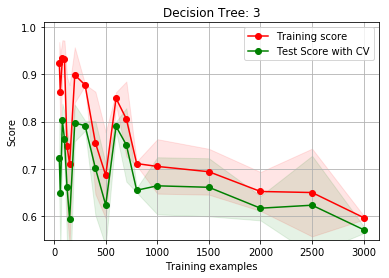
\includegraphics[width=1\textwidth,keepaspectratio]{1_curve_dtree3.png} 
      \caption*{Learning Curve for max\_depth = 3} 
   \endminipage\hfill
   \minipage{0.32\textwidth}
      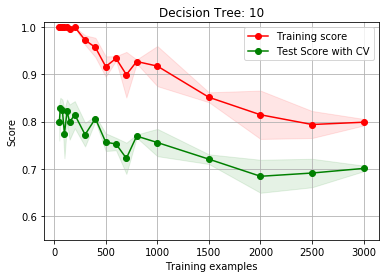
\includegraphics[width=1\textwidth,keepaspectratio]{1_curve_dtree10.png} 
      \caption*{Learning Curve for max\_depth = 10} 
   \endminipage\hfill
   \minipage{0.32\textwidth}
      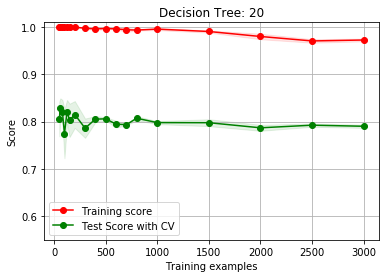
\includegraphics[width=1\textwidth,keepaspectratio]{1_curve_dtree20.png} 
      \caption*{Learning Curve for max\_depth = 20} 
   \endminipage\hfill
\end{figure}

\subsection*{Home Sale Prices}
\begin{tabular}{ | c | c | c | c | } 
\hline
\textbf{Max Depth} & \textbf{Train \%} & \textbf{Test \%} & \textbf{Runtime}  \\
\hline
cell1 dummy text dummy text dummy text& cell2 & cell3 \\ 
\hline
cell1 dummy text dummy text dummy text & cell5 & cell6 \\ 
\hline
cell7 & cell8 & cell9 \\ 
\hline
\end{tabular}


%
%\subsubsection*{Iteration 1}
%Centers: \{1, 6\} \\
%Cluster 1: \{1, 2, 3\} \\
%Cluster 2: \{4, 9, 12, 6, 10, 9\}
%\subsubsection*{Iteration 2}
%Cluster 1 Center: $(1 + 2 + 3) / 3 = 2$ \\
%Cluster 2 Center: $(4 + 9 + 12 + 6 + 10 + 9) / 6 = 8.33333333333$ \\ 
%Avg: $(2 + 8.33333333333) / 2 = 5.1666666666$\\ \\
%Centers: \{2, 8.33333333333\} \\
%Cluster 1: \{1, 2, 3, 4\} \\
%Cluster 2: \{9, 12, 6, 10, 9\}
%\subsubsection*{Iteration 3}
%Cluster 1 Center: $(1 + 2 + 3 + 4) / 4 = 2.5$ \\
%Cluster 2 Center: $( 9 + 12 + 6 + 10 + 9) / 5 = 9.2$ \\ 
%Avg: $(2.5 + 9.2) / 2 = 5.85$\\ \\
%Centers: \{2.5, 9.2\} \\
%Cluster 1: \{1, 2, 3, 4\} \\
%Cluster 2: \{9, 12, 6, 10, 9\}
%\subsection*{b)} 
%Yes, the algorithms has converged.  If you continued doing more iterations, the clusters would not change.
%
%\section*{2 - K-Means and Variance}
%\subsection*{a)}  
%The variance of a partition would go down since the furthest data points would realign with new clusters, allowing for a cluster to remove its furthest (and highest variance contributing) data point.
%\subsection*{b)} 
%A value of $n$ for k would \textbf{always} yield a variance of 0 because each instance would be aligned its own cluster.
%
%\section*{3 - Reinforcement Learning I}
%The reward function does not effectively communicate the goal to the agent.  By giving negative rewards per step taken and rewarding it for completion, you can train the agent to minimize the number of time spent in the maze and therefore have it complete the maze quicker.
%
%\section*{4 - Reinforcement Learning II}
%\subsection*{a)}  Only the intervals between the rewards are important.
%\subsection*{b)}
%$R_t=\sum_{k=0}^{\infty}\gamma^kr_{t+k+1}$ \\
%$V^\pi(s)=E_\pi[R_t \vert s_t = s]$\\
%$V^\pi(s)=E_\pi[\sum_{k=0}^{\infty}\gamma^kr_{t+k+1} \vert s_t = s]$\\ \\
%By adding constant C:\\
% $R_{t,c}=\sum_{k=0}^{\infty}\gamma^k[r_{t+k+1} + C]$ \\
% $=\sum_{k=0}^{\infty}\gamma^kr_{t+k+1} + \sum_{k=0}^{\infty}\gamma^kC$ \\
% $=R_t + \sum_{k=0}^{\infty}\gamma^kC$ \\
% $=R_t + \frac{C}{1-\gamma}$ \\
% $=R_t + K$ by setting $K = \frac{C}{1-\gamma}$ 
% 
% 

%\begin{figure}
%  \centering
%    \includegraphics[scale=.7]{skyscraper.jpg} 
%    \caption*{Skyscraper Base Image} 
%\end{figure}
%\begin{figure}
%  \centering
%    \includegraphics[scale=.7]{skyscraper4.jpg} 
%    \caption*{Skyscraper Segmented with K = 4} 
%\end{figure}
%\begin{figure}
%  \centering
%    \includegraphics[scale=.7]{skyscraper25.jpg} 
%    \caption*{Skyscraper Segmented with K = 25} 
%\end{figure}

\end{document}